%\listfiles
% Uncomment to make presentation file
%\documentclass[t,xcolor=pdftex,dvipsnames,table]{beamer}
% Uncomment to make handouts
%----------------------------------------------------------------------------%
\documentclass[t,xcolor=pdftex,dvipsnames,table,handout]{beamer}
\usepackage{pgfpages}
%\pgfpagesuselayout{4 on 1}[letterpaper,border shrink=5mm,landscape]
%----------------------------------------------------------------------------%


%\includeonlyframes{current}


\mode<presentation> {
  \usetheme{default}
    \definecolor{uofsgreen}{rgb}{.125,.5,.25} %
    \useoutertheme{default}
    \usecolortheme[named=uofsgreen]{structure}
  \setbeamercovered{transparent}
}

\mode<handout> {
    \setbeameroption{hide notes}
    }

\setbeamercolor{mybox}{bg=uofsgreen!20}

%%%%%%%%%%%%%%%%%%%%%%%%%%%%%%%%%%%%%%%%%%%%%%%%%%%%%%%%%%%%%%%%%%%%
% Include appropriate packages
%%%%%%%%%%%%%%%%%%%%%%%%%%%%%%%%%%%%%%%%%%%%%%%%%%%%%%%%%%%%%%%%%%%%
\usepackage{hyperref}
\hypersetup{
    colorlinks=true,
    linkcolor=blue,
    filecolor=magenta,      
    urlcolor=blue,
    pdftitle={Sharelatex Example},
    bookmarks=true,
    pdfpagemode=FullScreen,
}
\usepackage[english]{babel}
% or whatever
\usepackage[latin1]{inputenc}
% or whatever
\usepackage{times}
\usepackage[T1]{fontenc}
% Or whatever. Note that the encoding and the font should match. If T1
% does not look nice, try deleting the line with the fontenc.
\usepackage{colortbl}
\usepackage{tikz}
\usetikzlibrary{trees}
\usetikzlibrary{shapes}
%\usepackage{pgflibrarytikztrees}
    \definecolor{uofsgreen}{rgb}{.125,.5,.25}
%\usepackage{pgf}
%\usepackage{pgf,pgfarrows,pgfnodes,pgfautomata,pgfheaps}

    \graphicspath{{chapter24files/}}



\DeclareSymbolFontAlphabet{\mathcalold}{symbols}
\newcommand{\asum}[1]{\ensuremath{#1_1+#1_2+\cdots+#1_n}}
\newcommand{\avec}[1]{\ensuremath{#1_1,#1_2,\ldots,#1_n}}
\newcommand{\avecn}[2]{\ensuremath{#1_1,#1_2,\ldots,#1_{#2}}}
\newcommand{\asumn}[2]{\ensuremath{#1_1+#1_2+\cdots+#1_{#2}}}
\newcommand{\Bayes}{Bayes's}
\newcommand{\bd}{\begin{description}}
\newcommand{\bi}{\begin{itemize}}
\newcommand{\bnum}{\begin{enumerate}}
\newcommand{\bs}[1]{\ensuremath{\boldsymbol{#1}}}
\newcommand{\cnj}{\ensuremath{\phantom{}_nC_j}}
\newcommand{\cnja}[2]{\ensuremath{\phantom{}_#1C_#2}}
\newcommand{\cpdf}[3][p]{\ensuremath{\pdf[#1]{\left.#2\,\right|\,#3}}}
\newcommand{\dbar}{\ensuremath{\bar d}}
\newcommand{\df}{\ensuremath{\mbox{df}}}
\newcommand{\dfb}{\ensuremath{\mbox{df(between)}}}
\newcommand{\dfg}{\ensuremath{\mbox{df(groups)}}}
\newcommand{\dft}{\ensuremath{\mbox{df(total)}}}
\newcommand{\dfe}{\ensuremath{\mbox{df(error)}}}
\newcommand{\dfw}{\ensuremath{\mbox{df(within)}}}
\newcommand{\dis}{\displaystyle}
\newcommand{\ed}{\end{description}}
\newcommand{\enum}{\end{enumerate}}
\newcommand{\ei}{\end{itemize}}
\newcommand{\eps}{\ensuremath{\epsilon}}
\newcommand{\ie}{\emph{i.e.}}
\newcommand{\field}[1]{\mathbb{#1}}
\newcommand{\mc}[1]{{\ensuremath{\mathcal{#1}}}}
\newcommand{\mcc}[1]{\multicolumn{1}{c}{#1}}
\newcommand{\mcl}[1]{\multicolumn{1}{l}{#1}}
\newcommand{\mco}[1]{{\ensuremath{\mathcalold{#1}}}}
\newcommand{\mcr}[1]{\multicolumn{1}{r}{#1}}
\newcommand{\mr}[1]{{\ensuremath{\mathrm{#1}}}}
\newcommand{\MS}{\ensuremath{\mbox{SS}}}
\newcommand{\MSb}{\ensuremath{\mbox{MS(between)}}}
\newcommand{\MSg}{\ensuremath{\mbox{MS(groups)}}}
\newcommand{\MSt}{\ensuremath{\mbox{MS(total)}}}
\newcommand{\MSe}{\ensuremath{\mbox{MS(error)}}}
\newcommand{\MSw}{\ensuremath{\mbox{MS(within)}}}
\newcommand{\mb}[1]{{\ensuremath{\mathbf{#1}}}}
\newcommand{\mul}[3]{\multicolumn{#1}{#2}{#3}}
\newcommand{\model}{\mco I}
\newcommand{\MOE}{\ensuremath{\mbox{MOE}}}
\newcommand{\mud}{\ensuremath{\mu_d}}
\newcommand{\norm}[3]{\ensuremath{\mco N\left(#1\,\big|\,#2,\,#3\right)}}
\newcommand{\ntil}{\ensuremath{\tilde n}}
\newcommand{\pdf}[2][p]{\ensuremath{#1\left(#2\right)}}
\newcommand{\pfrac}[2]{\left(\frac{#1}{#2}\right)}
\newcommand{\phat}{\ensuremath{\hat p}}
\newcommand{\pstar}{\ensuremath{p^*}}
\newcommand{\ptil}{\ensuremath{\tilde p}}
\newcommand{\pval}{\ensuremath{\mbox{$P$-value}}}
\newcommand{\qhat}{\ensuremath{\hat q}}
\newcommand{\R}{\textsf{R}}
\newcommand{\simnorm}[2]{\ensuremath{\sim \mco N\left(#1,\,#2\right)}}
\newcommand{\SE}{\ensuremath{\mbox{SE}}}
\newcommand{\SEdiff}{\ensuremath{\mbox{SE}_{\bar{y}_1-\bar{y}_2}}}
\newcommand{\SEDiff}{\ensuremath{\mbox{SE}_{\bar{Y}_1-\bar{Y}_2}}}
\renewcommand{\SS}{\ensuremath{\mbox{SS}}}
\newcommand{\SSb}{\ensuremath{\mbox{SS(between)}}}
\newcommand{\SSt}{\ensuremath{\mbox{SS(total)}}}
\newcommand{\SSg}{\ensuremath{\mbox{SSG}}}
\newcommand{\SSe}{\ensuremath{\mbox{SSE}}}
\newcommand{\SSw}{\ensuremath{\mbox{SS(within)}}}
\newcommand{\sumin}{\ensuremath{\sum_{i=1}^{n}}}
\newcommand{\xbar}{\ensuremath{\bar x}}
\newcommand{\ybar}{\ensuremath{\bar y}}
\newcommand{\xbari}{\ensuremath{\bar x_{i}}}
\newcommand{\ybari}{\ensuremath{\bar y_{i}}}
\newcommand{\ybardd}{\ensuremath{\bar y_{\cdot\cdot}}}
\newcommand{\yij}{\ensuremath{y_{ij}}}
\newcommand{\Xbar}{\ensuremath{\bar X}}
\newcommand{\Ybar}{\ensuremath{\bar Y}}
%\renewcommand{\Pr}{{\ensuremath{\mathrm{Pr}(#1)}}}


%%%%%%%%%%%%%%%%%%%%%%%%%%%%%%%%%%%%%%%%%%%%%%%%%%%%%%%%%%%%%%%%%%%%
% Parameter specifications and image decs
%%%%%%%%%%%%%%%%%%%%%%%%%%%%%%%%%%%%%%%%%%%%%%%%%%%%%%%%%%%%%%%%%%%%


%%%%%%%%%%%%%%%%%%%%%%%%%%%%%%%%%%%%%%%%%%%%%%%%%%%%%%%%%%%%%%%%%%%%
% Set title and presentation information
%%%%%%%%%%%%%%%%%%%%%%%%%%%%%%%%%%%%%%%%%%%%%%%%%%%%%%%%%%%%%%%%%%%%

\title{Section 8.1: Analysis of Variance} % (optional, use only with long paper titles)
\subtitle{} % (optional)

\author{Eric D. Nordmoe}

\institute%
{Math 261\\
  Biostatistics\\
  Kalamazoo College}

\date{}


% If you wish to uncover everything in a step-wise fashion, uncomment
% the following command:

%\beamerdefaultoverlayspecification{<+->}

%----------------------------------------------------------------------------%
% Begin presentation frames
%----------------------------------------------------------------------------%

\newsavebox{\Imagebox}

\begin{document}

\begin{frame}
  \titlepage
\end{frame}

%----------------------------------------------------------------------------%
\begin{frame}{Outline}
\bi
    \item Overview of Analysis of Variance
    \item The Basic ANOVA
    \item The ANOVA Model
    \item Checking Conditions
\ei
\end{frame}
%----------------------------------------------------------------------------%
\begin{frame}{The Basic Idea of ANOVA}
\begin{block}{}

When we ask if a set of sample means gives evidence for \alert{differences
among the population means}, what matters is not how far apart the
sample  means are but how far apart they are \alert{relative to the
variability of individual observations}.\\[1ex]
\hfill{\emph{Baldi \& Moore, 3rd ed., p.606}}
\end{block}
\end{frame}
%----------------------------------------------------------------------------%
\begin{frame}{The Basic Idea of ANOVA}
\begin{block}{}
The basic idea is to compare measures of variability, both
    \alert{between} the groups and \alert{within} each group, as a way to assess how
    different the groups really are.\\[1ex]
\hfill{\emph{Lock5, p.540}}
\end{block}
\end{frame}
%----------------------------------------------------------------------------%
\begin{frame}{Analysis of Variance Sampling Model}
Draw \alert{simple random samples} from $k$ \alert{independent} populations to compare
population means $\mu_1$, $\mu_2$, $\ldots$, and $\mu_k$:
    \vspace{-1ex}
\begin{center}
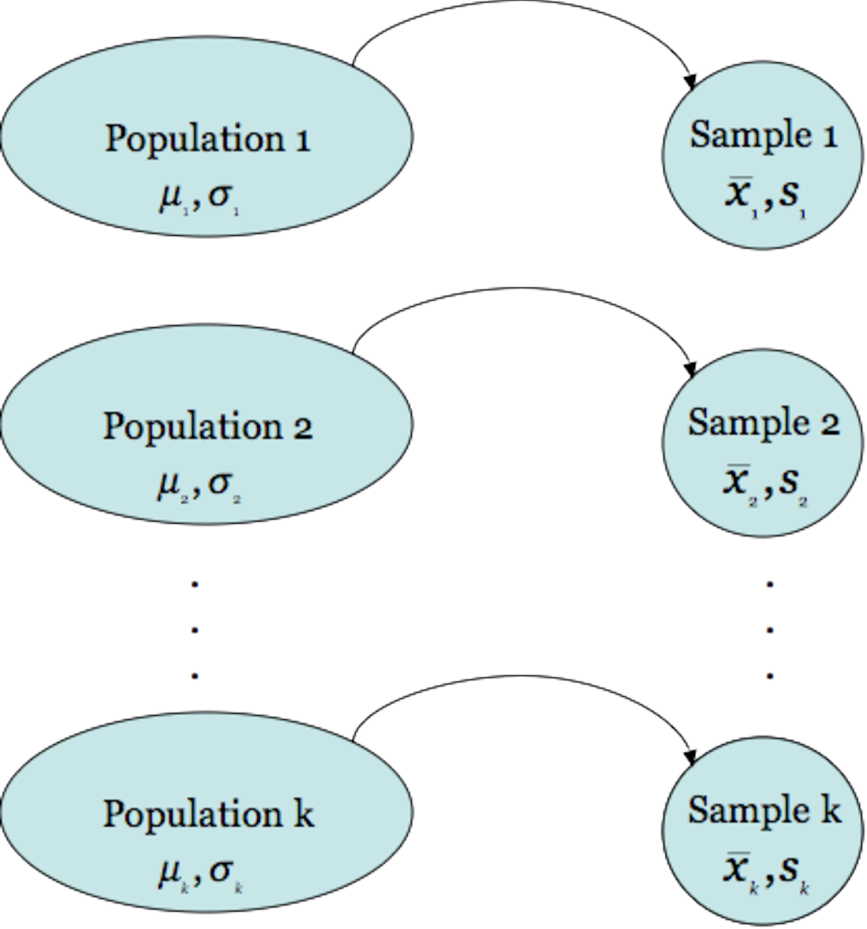
\includegraphics[height=2.5in]{sampling_model.pdf}
\end{center}
\pause
 \vspace{-1ex} Condition: $\sigma_1=\sigma_2=\cdots=\sigma_k=\sigma$
\end{frame}
%----------------------------------------------------------------------------%
\begin{frame}{Conditions for Applying ANOVA}
  \begin{enumerate}
    \item We have \alert{$k$ independent SRSs}, one from each of $k$ populations.\pause
      \item Each of the $k$ populations has a \alert{Normal
          distribution} with   an unknown mean $\mu_i$. \pause
        \item All of the populations  have the \alert{same standard deviation}  $\sigma$, whose value is unknown.
  \end{enumerate}
\end{frame}
%----------------------------------------------------------------------------
\begin{frame}{Case Study}
\framesubtitle{Diet Restriction and Longevity}
\bi
    \item  Study of the effect
of restricting caloric intake on life expectancy. \pause
    \item Female mice randomly assigned to one of 6 treatment
    groups:
    \begin{enumerate}
        \item \alert{NP:} unlimited nonpurified standard diet for
        laboratory mice. \pause
        \item   \alert{N/N85 (control group):} fed normally both before and after
        weaning. Caloric intake controlled at 85 kcal/wk after
        weaning. \pause
        \item \alert{N/R50:} normal diet before weaning and
        reduced-calorie diet of 50 kcal/wk after weaning. \pause
        \item \alert{R/R50:} reduced-calorie diet of 50 kcal/wk
        before and after weaning. \pause
        \item \alert{N/R50 lopro:} normal diet before weaning,
        restricted diet of 50 kcal/wk after weaning with dietary
        protein content decreased with advancing age. \pause
        \item \alert{N/R40:} normal diet before weaning, severely
        reduced-calorie diet of 50 kcal/wk after weaning.
    \end{enumerate}
    \pause
    \item Several questions of interest to be addressed.

 \ei

\end{frame}
% ----------------------------------------------------------------------------%
\begin{frame}{Case Study}
  \framesubtitle{Diet Restriction and Longevity: Study Citation}
 
Weindruch R, Walford RL, Fligiel S, Guthrie D. The retardation of
aging in mice by dietary restriction: longevity, cancer, immunity and
lifetime energy intake. \emph{J
Nutr.} 1986;116(4):641-654. doi:10.1093/jn/116.4.641

\end{frame}
% ----------------------------------------------------------------------------%


\begin{frame}{Planned Comparisons Among Groups in the Diet
Restriction Study}

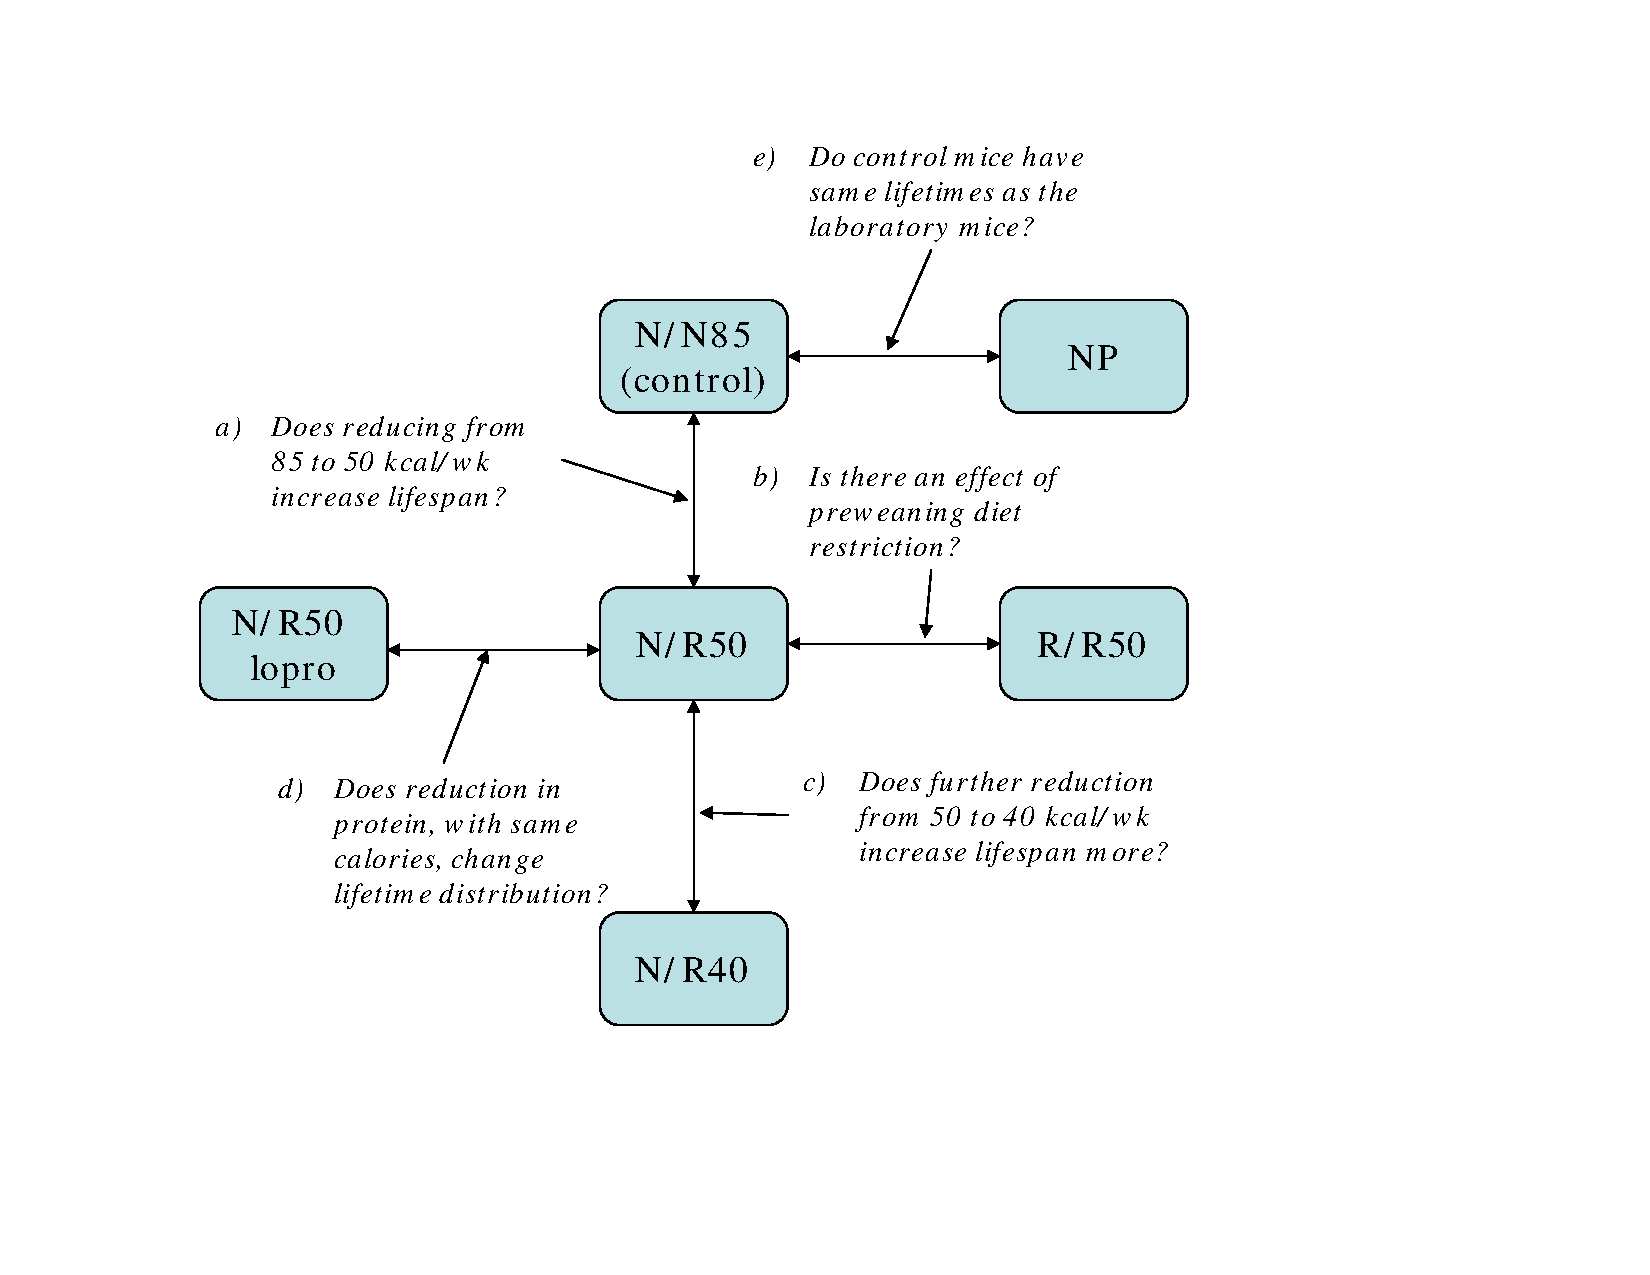
\includegraphics[height=3in]{planned_comps.pdf}


\end{frame}
%----------------------------------------------------------------------------%
\begin{frame}{Diet Restriction Study}
\framesubtitle{Exploratory Plots}

\begin{block}{}
Use R to create plots to explore the possibility of differences
among the means.
\end{block}
\end{frame}
%----------------------------------------------------------------------------%
\begin{frame}{The Big Picture of ANOVA}
\bi
    \item \alert{Key question:} Is variability \alert{across} populations
    greater than variability \alert{within} populations
    \bi
        \item Variability \alert{between} vs \alert{within}
    \ei
    \pause
    \item \alert{Hypothesis test:}
    \bi
        \item $H_0:\mu_1=\mu_2=\cdots=\mu_k$ versus \pause
        \item $H_a: \mbox{At least one } \mu_i\neq\mu_j$
    \ei
    \pause
    \item \alert{Test statistic ($F$):} ratio of the variability
      \alert{among} group (or treatment)
means over the variability \alert{within} samples.
$$
F=\frac{\mbox{variation among the sample means}}{\mbox{variation among
    individuals in the same sample}}
$$
    \bi
        \item Large test statistic $\Rightarrow$ evidence against
        $H_0$
        \note{Note that the nature of the test statistics will be
        different here. It will focus on variability rather than on
        means directly. Note that it's due to Fisher.}
    \ei
    \pause
    \item Results are summarized in the ANOVA table.
    \note{Accounting table for computing the test statistics by
    apportioning variability across the various possible sources.}

\ei

\end{frame}
%----------------------------------------------------------------------------%
\begin{frame}{Notation}
Key notation used in calculations for comparing variability
\alert{between groups} and \alert{within groups}:
\begin{eqnarray*}
k & = & \mbox{number of groups} \\
  n_i &=& \mbox{sample size for group $i$}\\
  \xbari &=&  \mbox{sample mean for group $i$} \\
  s_i &=&  \mbox{standard deviation for group $i$} \\
  n &=& \sum_{i=1}^{k}n_i = \mbox{total sample size} \\
  \xbar &=&  \frac{\sum_{i=1}^{k}n_i
  \xbari}{n}=
  \mbox{overall mean}.
\end{eqnarray*}
\end{frame}
%----------------------------------------------------------------------------%
\begin{frame}{Apportioning Variability}
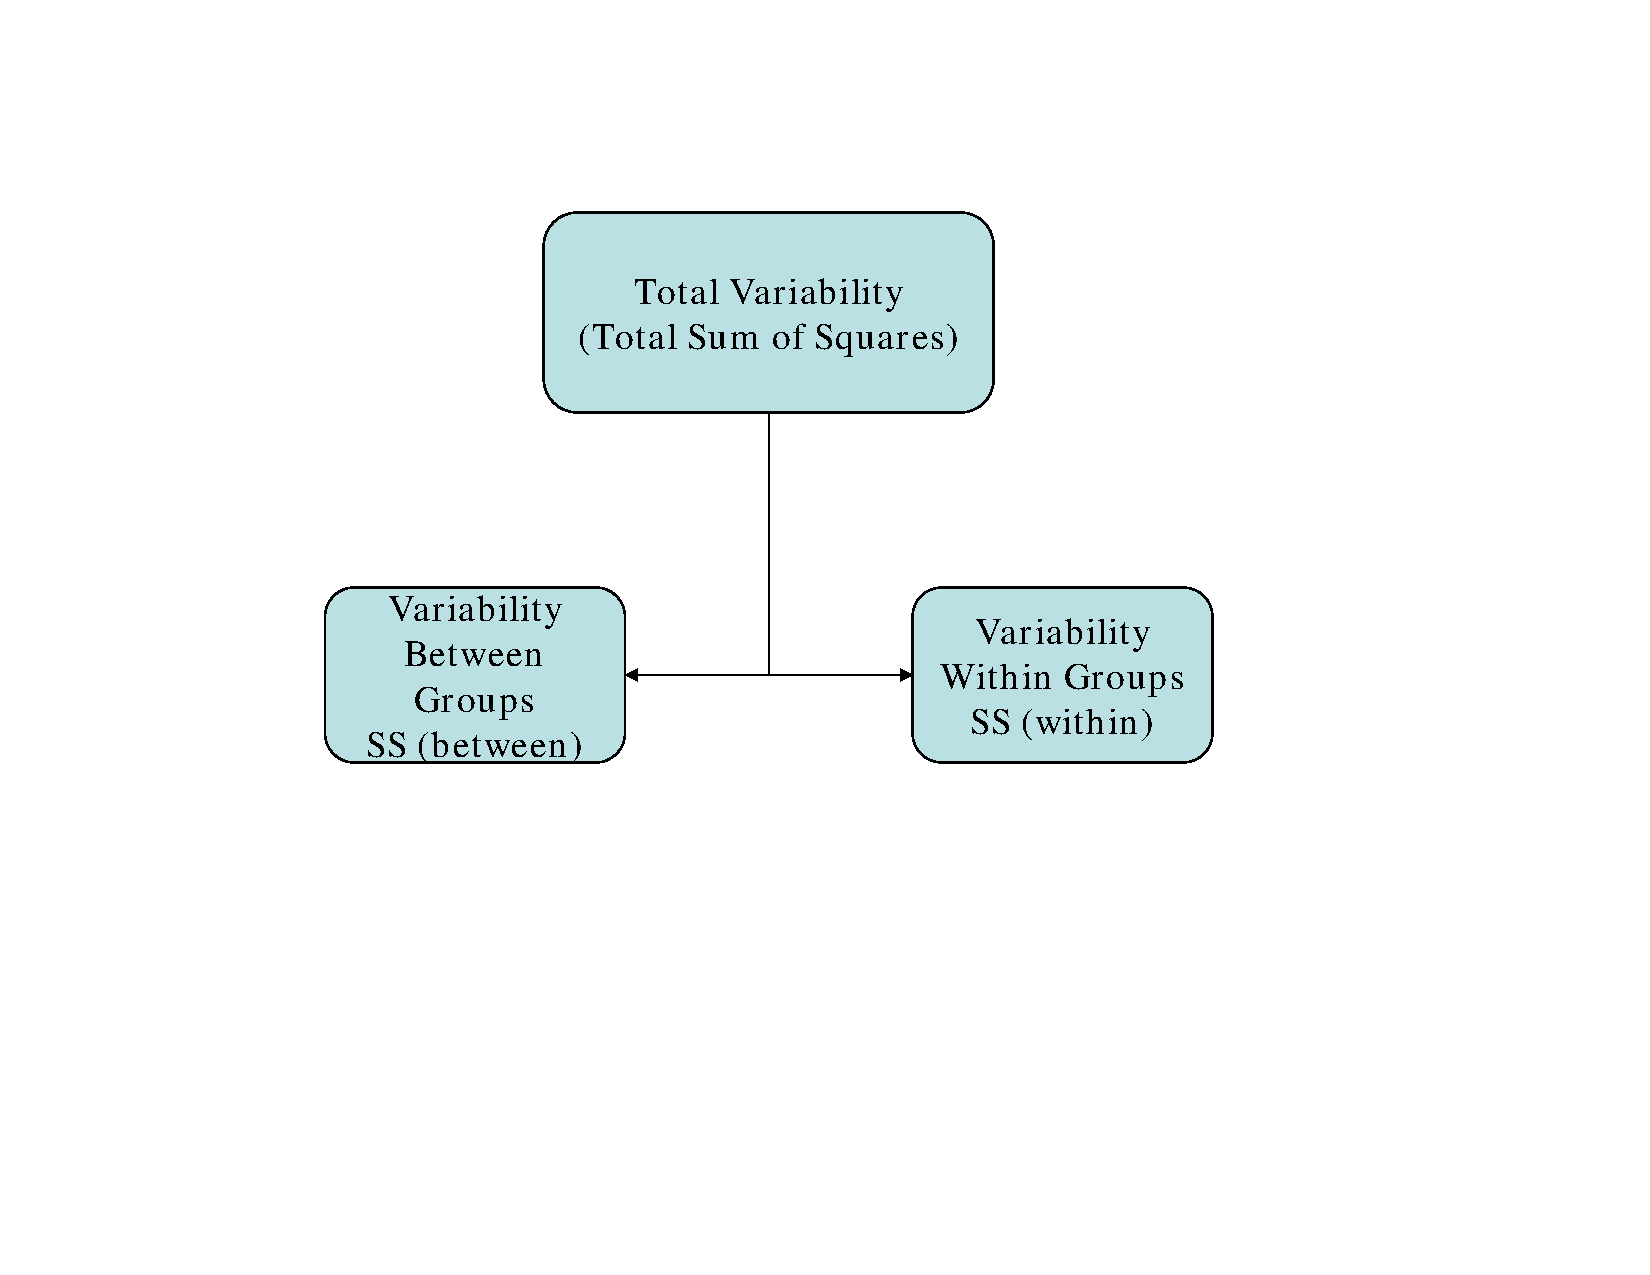
\includegraphics[height=2.5in]{sumofsquares.pdf}
\end{frame}
%----------------------------------------------------------------------------%
\begin{frame}{Variability within Groups}
Measure \alert{variability within groups} by the sum of squared
deviations from the group mean:
$$
  \SSe =  (n_1-1) s_1^2 +(n_2-1) s_2^2 +\cdots +(n_k-1) s_k^2 
$$
\note{$\SSe$ is a \emph{weighted sum} of the sample variances where
the weights are the \emph{degrees of freedom} for each group.}
\end{frame}
%----------------------------------------------------------------------------%
\begin{frame}{Degrees of Freedom}
\bi
    \item The \alert{degrees of freedom within} samples is the sum of
degrees of freedom for each sample.\pause
\begin{eqnarray*}
\dfe&=& (n_1-1)+(n_2-1)+\cdots+(n_k-1)\\
&=& n-k
\end{eqnarray*}
\pause
    \item This is also equal to the total sample size minus the
    number of groups.
\ei
\end{frame}
%----------------------------------------------------------------------------%
\begin{frame}{Mean Square within Groups (Error)}
In ANOVA, the \alert{mean square} measures variability as the ratio
of \alert{sum of squares} to \alert{degrees of freedom.}

\begin{eqnarray*}
% \nonumber to remove numbering (before each equation)
 \mbox{MSE}= \MSe &=& \frac{\SSe}{\dfe} \\
    &=& \frac{(n_1-1)s_1^2+\cdot+(n_I-1)s_k^2}{n-k}
\end{eqnarray*}
    \note{Note that $\MSe$ is a weighted average of the
    group-specific sample variances.}
    \pause
 \bi
    \item The \alert{pooled standard deviation ($s_p$)} estimates the
    common group-specific standard deviation:
    $$
        s_p = \sqrt{\MSe}
    $$
    \ei
\end{frame}
%----------------------------------------------------------------------------%
\begin{frame}{Variability between Groups}
Measure \alert{variability between groups} by $\SSb$, a weighted sum
of squared deviations of group means from the grand mean:
$$
  \SSg =  n_1 (\xbar_1-\xbar)^2+n_2 (\xbar_2-\xbar)^2+ \cdots+n_k (\xbar_k-\xbar)^2
$$
\pause

The corresponding \alert{degrees of freedom between groups} is one
less than the number of groups:
$$
\dfg=k-1
$$
\end{frame}
%----------------------------------------------------------------------------%
\begin{frame}{Mean Square between Groups}
The mean square between groups, MSG or MS (treatment) is the \alert{ratio} of the sum of squares over the
degrees of freedom:
\begin{eqnarray*}
\mbox{MSG} &=& \frac{\SSg}{\dfg} \\
        &=& \frac{n_1 (\xbar_1-\xbar)^2+n_2 (\xbar_2-\xbar)^2+ \cdots+n_k (\xbar_k-\xbar)^2}{k-1}
\end{eqnarray*}
\end{frame}
%----------------------------------------------------------------------------%
\begin{frame}{The $F$ Statistic}
\bi
    \item The $F$ statistic is the ratio of the \alert{mean square between}
    to the \alert{mean square within.}
    $$
        F= \frac{\mbox{MSG}}{\mbox{MSE}}
    $$
    \item If the null hypothesis is true, $F$ has an $F$
    distribution with \alert{$k-1$} and \alert{$n-k$} degrees of freedom
    \note{ This assumes the conditions of the test are met.}
    \pause
    \item Use the StatKey  $F$ distribution web applet to find
      $p$-values when necessary or obtain them from R output for
      ANOVA using the \textbf{lm()} command we also used for regression.

 \ei
 \end{frame}
%----------------------------------------------------------------------------%
\begin{frame}{Diet Restriction Study}
See \href{https://heroic-horse-92e142.netlify.app/r_commands_for_anova}{R Commands for ANOVA} for R help.

\end{frame}
% -------------------------------------------------------------------%
\begin{frame}
  \vskip25mm
  \centering \begin{block}
  {\Huge Checking Conditions}
\end{block}
\end{frame}

  
%----------------------------------------------------------------------------%
\begin{frame}{Analysis of Variance Sampling Model}
Draw samples from $k$ \alert{independent} populations to compare
population means $\mu_1$, $\mu_2$, $\ldots$, and $\mu_k$:
    \vspace{-1ex}
\begin{center}
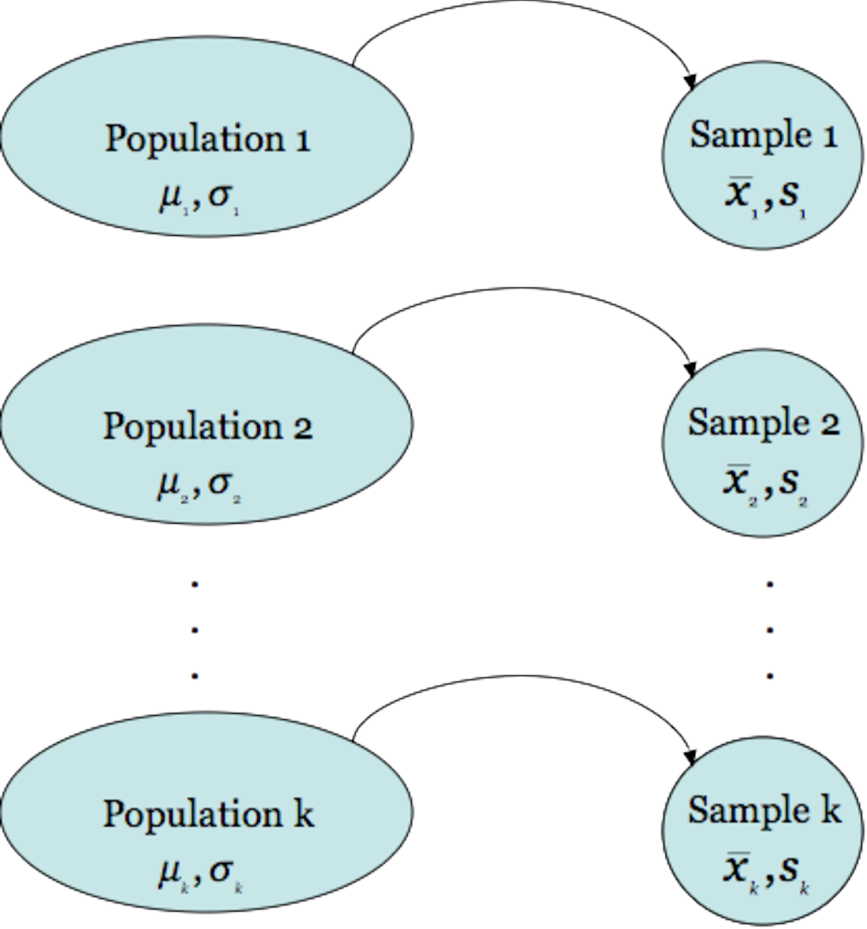
\includegraphics[height=2.5in]{sampling_model.pdf}
\end{center}
 \vspace{-1ex} Condition: $\sigma_1=\sigma_2=\cdots=\sigma_k=\sigma$
\end{frame}
%----------------------------------------------------------------------------%
\begin{frame}{Standard Conditions for ANOVA}
\bi
    \item \alert{Design conditions:}
    \bi
        \item \alert{Random samples:} reasonable to consider observations
        a random sample from respective populations \pause
        \item \alert{Independent samples:} the $k$ samples are
        independent of each other
        \note{Matched pair designs do not fit within the context of
        ANOVA but are incorporated in randomized block designs.}
    \ei
    \pause
    \item \alert{Population:}
    \bi
        \item \alert{Normal:} Population distributions are normal
        \pause
        (not crucial if $n_i$ are large and similar)
        \pause
        \item \alert{Equal standard deviations:}
        $$
            \sigma_1=\sigma_2=\cdots=\sigma_k=\sigma
        $$
    \ei
\ei
\end{frame}

%----------------------------------------------------------------------------%
\begin{frame}{Rules of Thumb for Checking ANOVA Conditions}
\bi
    \item Inference requires \alert{random samples}.\pause
    \item \alert{Outliers} are always problematic! Plot your data.
    \pause
    \item ANOVA methods are robust if group samples sizes are \alert{similar and
    not too small}. \pause
    \item Ratio of largest sample SD to smallest should not be much
    greater than \alert{2}. \pause
    \bi
        \item Biggest \alert{problem} is if sample sizes are \alert{unequal} and SD
        from a small sample is \alert{much larger} than others.
    \ei
    \pause
    \item Normality is not critical if sample sizes $n_i$ are
    \alert{large} and approximately \alert{equal}.
\ei
\end{frame}
%----------------------------------------------------------------------------%

%----------------------------------------------------------------------------%
\end{document}


%Following draws a thin line 6 cm long
%\rule{6cm}{.01cm}

%%% Local Variables:
%%% mode: latex
%%% TeX-master: t
%%% End:
